\section{Theorie}
\label{sec:Theorie}



\subsection{Aufbau einer Kathodenstrahlröhre}

Eine Kathodenstrahlröhre besteht aus einer Elektronenkanone, einem Ablenksystem und einem Nachweissystem.

\begin{figure}[H]
  \centering
  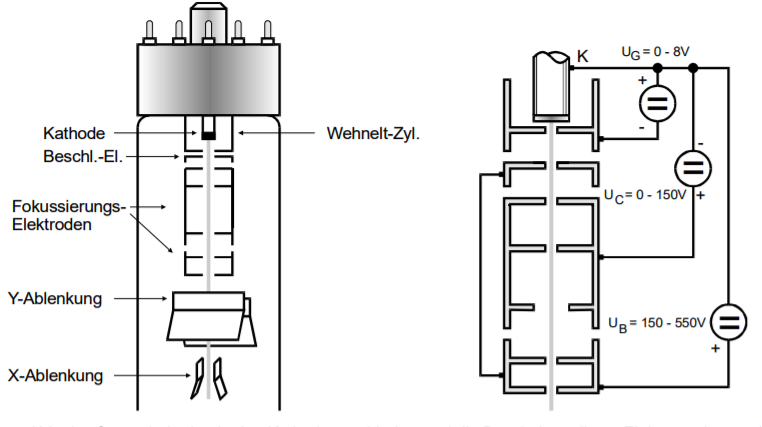
\includegraphics[height=8cm]{kathodenstrahlroehre.PNG}
  \caption{Aufbau einer Kathodenstrahlröhre(links) und Beschaltung einer Elektronenkanone (rechts)}
  \label{fig:kathode}
\end{figure}

Durch Glühemission werden freie Elektronen erzeugt. Die Kathode wird über einen, mit Strom durchflossenen, Draht
erhitzt.
Mit dem negativen Potenzial des Wehnelt-Zylinders, welcher die Kathode umgibt, kann die
Intensität des Elektronenstrahls gesteuert werden.
Die vor dem Wehnelt-Zylinder liegende Elektrode besitzt ein hohes positives Potenzial gegenüber der Kathode
und beschleunigt die Elektronen auf die Geschwindigkeit $v_z$.
Aus dem Energiesatz folgt:
\begin{equation}
  \frac{m_0 v_z^2}{2} = e_0 U_B
  \label{eqn:energie}
\end{equation}

Die inhomogenen elektrischen Felder der Fokussierungselektroden bündeln den Elektronenstrahl, welcher dann
auf den Leuchtschirm fällt. Dadurch werden Aktivatorzellen angeregt und emmittieren Lichtquanten.
Der Auftreffpunkt des Strahls wird somit sichtbar.

Das Ablenksystem wird von dem Elektronenstrahl auf dem Weg zum Leuchtschirm durchlaufen. Es besteht aus
zwei Plattenpaaren die senkrecht aufeinander stehen. Wird eine elektrische Spannung an diese Platten angelegt, übt das
elektrische Feld eine Kraft auf die Elektronen aus, welche daraufhin abgelenkt werden.
Der Leuchtfleck auf dem Bildschirm verschiebt sich.

\subsection{Ablenkung eines Elektronenstrahls im E-Feld}

\begin{figure}[H]
  \centering
  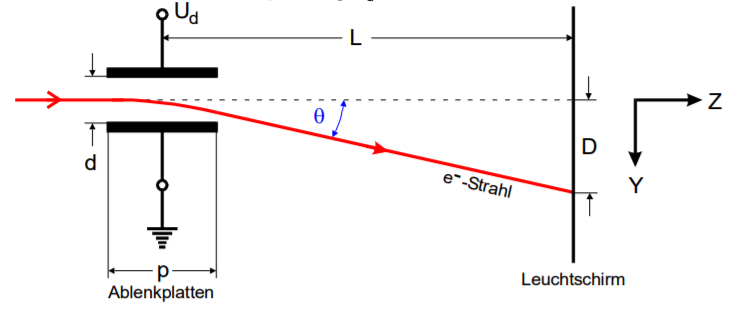
\includegraphics[height=8cm]{ablenkungefeld.PNG}
  \caption{Ablenkung des Strahls durch das Ablenksystem}
  \label{fig:ablenkung}
\end{figure}

Wenn der Plattenabstand $d$ klein gegenüber der Plattenlänge $p$ ist, so wird zwischen den Platten
ein homogenes elektrisches Feld angenommen. Dessen Feldstärke beträgt:
\begin{equation}
  E = \frac{U}{d}
\end{equation}

Auf ein Elektron wird dann im homogenen E-Feld die Kraft:
\begin{equation}
  |\vec{F}| = |e_0 \vec{E}| = e_0 \frac{U_d}{d}
\end{equation}

Die Geschwindigkeit in Y-Richtung ist dann:
\begin{equation}
  v_y = \frac{F}{m_0} \Delta t
\end{equation}

Da die Elektronen weiterhin die Geschwindigkeit $v_z$ in Z-Richtung haben, gilt für
die Durchlaufdauer $\Delta t$ des E-Feldes:
\begin{align}
  \Delta t = \frac{p}{v_z}
\end{align}

Mit Gleichung (3) und (4) folgt für $v_y$:
\begin{align}
  v_y = \frac{e_0}{m_0} \frac{U_d}{d} \frac{p}{v_z}
\end{align}

Der Winkel $\Theta$ des Elektronenstrahls nach dem Durchlaufen des E-Feldes ist $\Theta = \frac{v_y}{v_z}$.
Für die Verschiebung $D$ des Leuchtfleckes gilt dann:
\begin{equation}
  D = L \Theta = \frac{e_0}{m_0} L \frac{U_d}{U_B}
\end{equation}
 Mit Gleichung \eqref{eqn:energie} folgt:
\begin{equation}
  D = \frac{p}{2d} L \frac{U_d}{U_B}
\end{equation}

Die Verschiebung $D$ ist somit proportional zu zur Ablenkspannung $U_d$.

\subsection{Kathodenstrahl-Oszillograph}

Um eine Kathodenstrahlröhre zu einem Kathodenstrahl-Oszillograph zu erweitern wird eine
Sägezahnspannung an die Ablenkplatten für die horizontale Ablenkung angelegt. Dieser
kann die Zeitabhängigkeit von Wechselspannungen darstellen.
Stehen die Frequenzen der beiden Spannungen in einem geeigneten Verhältnis gilt:
\begin{equation}
  n \nu_S = m \nu_W
\end{equation}


\subsection{Elektronenbahnen im homogenen Magnetfeld}

Bewegt sich ein Teilchen mit der Ladung $q$ und der Geschwindigkeit $\vec{v}$ im homogenen Magnetfeld $\vec{B}$, so
wirkt die Lorentz-Kraft $F_L$ auf dieses Teilchen.
\begin{equation}
  F_L = q \vec{v} \times \vec{B}
\end{equation}

Die Bahn des Teilchen wird zu einer Kreisbahn, wenn die Bewegungsrichtung komplett senkrecht auf der
Richtung des Magnetfeldes steht.
Der Krümmungsradius $r$ ist durch das Gleichgewicht von Lorentzkraft und Zentrifugalkraft festgelegt.
\begin{align}
  e_0 v_0 B = \frac{m_0 | \vec{v} |^2}{r}
\end{align}

Da $|v| = v_0$ gilt, folgt daraus:
\begin{equation}
  r = \frac{m_0 v_0}{e_0 B}
\end{equation}

Die rechte Seite ist konstant und somit auch der Krümmungsradius.


\subsection{Bestimmung der spezifischen Elektronenladung}

\begin{figure}[H]
  \centering
  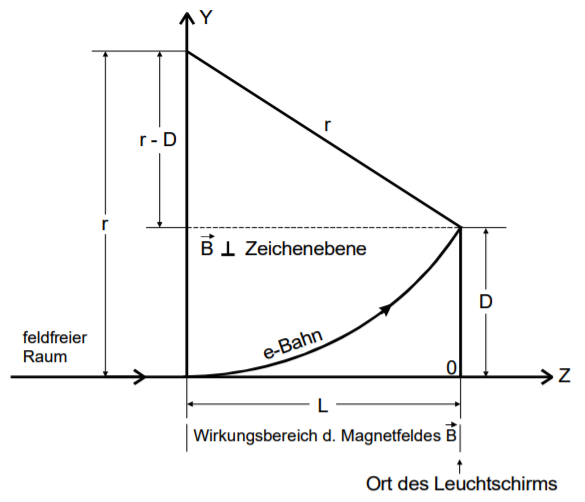
\includegraphics[height=8cm]{ablenkungbfeld.PNG}
  \caption{Ablenkung des Strahls im Magnetfeld}
  \label{fig:ablenkungbfeld}
\end{figure}

Aus der Abbildung (3) kann der Krümmungsradius mit dem Satz des Pythagoras bestimmt werden.
Es gilt:
\begin{equation}
  L^2 + (r - D)^2 = r^2
\end{equation}

Aus Gleichung (12) folgt daraus:
\begin{equation}
  \frac{L^2 + D^2}{2D} = \frac{m_0 v_0}{e_0 B}
\end{equation}

Ist $U_B$ ein Beschleunigungspotenzial der Kathodenstrahlröhre, so gilt nach dem Energiesatz:
\begin{equation}
  v_0 = \sqrt{2U_B e_0/m_0}
\end{equation}

Daraus folgt für Gleichung (14):
\begin{equation}
  \frac{L^2 + D^2}{2D} = \frac{m_0}{e_0 B} \sqrt{2U_B e_0/m_0}
\end{equation}

Die magnetische Flussdichte des Helmholtz-Feldes ist im Innern des Spulenpaares wie folgt definiert:
\begin{equation}
  B = \mu_0 \frac{8}{\sqrt{125}} \frac{NI}{R}
\end{equation}

Wobei $R$ der Spulenradius, $N$ die Windungszahl, $\mu_0$ die magnetische Feldkonstante und
$I$ der Spulenstrom ist.
